\section{Theorie}
\label{sec:Theorie}

\subsection{Drehimpuls und magnetisches Moment in der Elektronenhülle}
\label{subs:Drehimpuls und magnetisches Moment in der Elektronenhülle}

Aus dem Gesamtdrehimpuls $J$ der Elektronenhülle resultiert ein magnetisches Moment $\vec \mu_\text{J}$, welches über
\begin{equation}
  \big \vert \vec \mu_\text{J}\big \vert=g_\text{J}\mu_\text{B} \sqrt{J(J+1)}
\end{equation}
bestimmt werden kann. Dabei ist $\mu_\text{B}$ das Bohrsche Magneton und $g_\text{J}$ der Landé-Faktor.
Da $\vec\mu_\text{J}$ sich aus dem magnetischen Moment des Bahndrehimpulses und des Spins zusammensetzt, gilt für schwache Magnetfelder
\begin{equation}
  \vec\mu_\text{J}=\vec\mu_\text{L}+\vec\mu_\text{S}.
\end{equation}
Diese lassen sich über
\begin{align}
  &\big \vert\vec \mu_\text{L}\big \vert=\mu_\text{B} \sqrt{L(L+1)} ~~~~~~\text{und}\\
  &\big \vert\vec \mu_\text{S}\big \vert=g_\text{S}\mu_\text{B} \sqrt{S(S+1)}
\end{align}
berechnen. Im zweiten Ausdruck steht das $g_\text{S}$ für den Landé-Faktor des freien Elektrons und hat einen Wert von $g_\text{S}=2,00232$.
\begin{figure}[H]
	\centering
	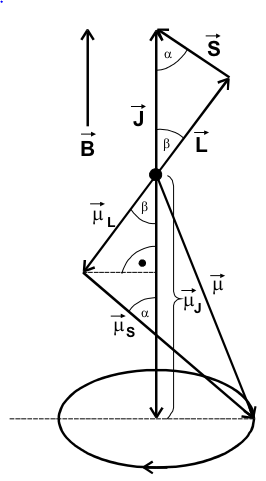
\includegraphics[width=5cm]{abb1.jpg}
	\caption{Zusammenhang Drehimpuls und magnetisches Moment der Valenzelektronen \cite{V21}}
	\label{abb:abb1}
\end{figure}
In Abbildung \ref{abb:abb1} wird verdeutlicht, dass das Gesamtmoment um die $\vec J$-Achse präzidiert, sodass sich eine parallele und eine senkrechte Komponente des magnetischen Moments ergibt.
Dabei ist zu beachten, dass die senkrechte Komponente sich zeitlich herausmittelt. Mit dem Ansatz
\begin{equation}
  \big \vert\vec \mu_\text{J}\big \vert=\big \vert\vec \mu_\text{L}\big \vert\cos{\beta}+ \big \vert\vec \mu_\text{S}\big \vert \cos{\alpha}
\end{equation}
kann unter Zuhilfenahme der geometrischen Relationen, die in Abbildung \ref{abb:abb1} erkennbar sind und mit dem Kosinussatz der Ausdruck
\begin{equation}
  g_\text{J}=\frac{3,0023J(J+1)+1,0023[S(S+1)-L(L+1)]}{2J(J+1)}
\end{equation}
zur berechnung des Landé-Faktors des Gesamtdrehimpulses hergeleitet werden.
Durch den Einfluss eines äußeren Magnetfeldes können die Energieniveaus verändert werden. Die Wechselwirkungenergie beträgt dabei
\begin{equation}
  U_\text{mag}=-\vec\mu_\text{J} \vec B.
\end{equation}
Auch hier mittelt sich die senkrechte Komponente aufgrund der Präzission heraus. Zusätzlich können nur ganzzahlige Vielfache $M_\text{J}$ angenommen werden. Aus diesem Grund ändert sich der Ausdruck der
Wechselwirkungsenergie zu
\begin{equation}
  U_\text{mag}=M_\text{J}g_\text{J}\mu_\text{B}B ~~~~\text{mit -J, -J+1, ..., J-1, J}
\end{equation}
Das Phänomen der Aufspaltung in $2J+1$ Energieniveaus unter Einfluss eines äußeren Magnetfeldes wird als Zeeman-Effekt bezeichnet.

\subsection{Einfluss des Kernspins bei Alkali-Atomen}

Für die im Versuch zu untersuchenden Atome muss der Gesamtdrehimpuls angepasst werden, da die Atome einen Kernspin besitzen. Es tritt eine weitere Aufspaltung der Energieniveaus auf, die sogenannte Hyperfeinstruktur,
welche auch die Aufspaltung durch den Zeeman-Effekt beeinflusst. Bei schwachen Magnetfeldern gilt
\begin{equation*}
  \vec F = \vec J + \vec I.
\end{equation*}
Auch das so entstehende magnetische Moment des Kerns ist gequantelt. Es ergeben sich entweder $2J+1$ beziehungsweise $2I+1$ Hyperfeinstrukturterme, falls $J < I$ oder $J > I$.
Für diese Hyperfeinstrukturterme wird die Quantenzahl $F$ eingeführt, die von $I+1$ bis $\vert I-J\vert$ läuft.
Im Falle eines Alkali-Atoms gilt $J=\frac{1}{2}$ und $I=\frac{3}{2}$, daraus folgt direkt, dass $F$ zwei Werte annehmen kann und somit eine Aufspaltung in zwei Niveaus stattfindet.
Mit einem externen Magnetfeld kann zusätzlich eine Aufspaltung in $2F+1$ Niveaus erzeugt werden. Ein Beispiel dafür ist in Abbildung \ref{abb:abb2} zu sehen.
\begin{figure}[H]
	\centering
	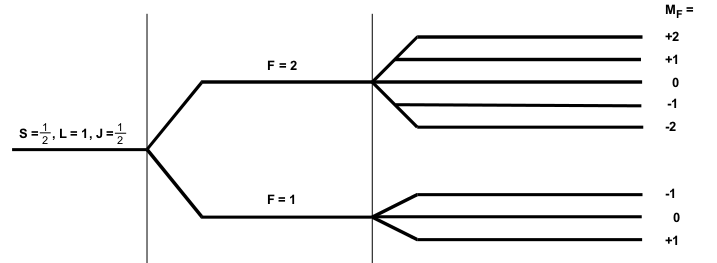
\includegraphics[width=12cm]{abb2.jpg}
	\caption{Beispiel für die Hyperfeinstrukturaufspaltung und die Zeeman-Aufspaltung eines Alkali-Atoms mit Kernspin \cite{V21}}
	\label{abb:abb2}
\end{figure}
Analog zur Berechnung des Landé-Faktors ohne Berücksichtigung des Kernspins kann mit dem Ansatz
\begin{equation}
  \big \vert \mu_\text{F} \big \vert = \sqrt{F(F+1)}
\end{equation}
ein Ausdruck für den Landé-Faktor mit Berücksichtigung des Kernspins gefunden werden. Dieser hat die Form
\begin{equation}
  g_\text{F}=g_\text{J}\frac{F(F+1)+J(J+1)-I(I+1)}{2F(F+1)}.
\end{equation}

\subsection{Optisches Pumpen}

Mit der Methode des optischen Pumpens soll ein Niveau des Atoms vollständig leergepumpt werden. Zuerst wird die Zeeman-Aufspaltung des Atoms wieder ohne Kernspinn betrachtet. Da sowohl für den $^2S_\frac{1}{2}$ Zustand
als auch für den $^2P_\frac{1}{2}$ Zustand $J=\frac{1}{2}$ gilt, werden beide Linien in zwei aufgespaltet. Diese Aufspaltung ist in Abbildung \ref{abb:abb3} schematisch dargestellt. Auch die Übergangsmöglichkeiten,
welche aus den Auswahlregeln $\Delta M=0, \pm 1$ resultieren, sind in der Abbildung eingetragen.
\begin{figure}[H]
	\centering
	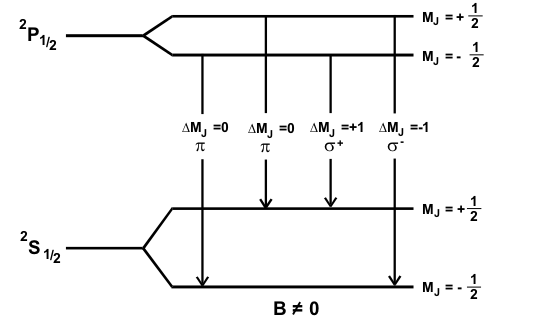
\includegraphics[width=12cm]{abb3.jpg}
	\caption{Zeeman-Aufspaltung der Energieniveaus ohne Kernspinn und Übergangsmöglichkeiten \cite{V21}}
	\label{abb:abb3}
\end{figure}
Diese können auch optisch auseinander gehalten werden, da sie unterschiedliche Polarisationen besitzen. Es wird unterschieden zwischen dem $\sigma^+$-Übergang mit $\Delta M_\text{J}=+1$, der rechtszirkular-polarisiertem
Licht entspricht und daher die Lichtquanten antiparallel zur Ausbreitungsrichtung sind und zwischen dem $\sigma^-$-Übergang mit $\Delta M_\text{J}=-1$, bei dem Spin und Ausbreitungsrichtung parallel verlaufen. Zusätzlich
sind noch die $\pi$-Übergänge mit $\Delta M_\text{J}=0$ vorhanden. Bei diesen wird linear polarisiertes Licht abgestrahlt und die Abstrahlungsintensität senkrecht zum $B$-Feld ist maximal.
Bei den $\sigma$-Übergängen ist dies anders. Hier ist nur in $B$-Feldrichtung das licht zirkular polarisiert, parallel zu dieser Richtung jedoch linear.
In der Ausgangslage, nachdem die Niveaus aufgespalten wurden, befinden sich alle Atome im Grundzustand. Das $M_\text{J}=-\frac{1}{2}$-Niveau ist dabei etwas mehr besetzt als das $M_\text{J}=+\frac{1}{2}$-Niveau.
Mit Hilfe eines Polarisationfilters und einer $\lambda /4$-Platte kann rechtszirkular-polarisiertes $D_1$-Licht erzeugt werden. Aufgrund der Auswahlregel $\Delta M_\text{J}=+1$ ist nur ein Übergang vom
$^2S_\frac{1}{2}$, $M_\text{J}=-\frac{1}{2}$ Niveau zum $^2P_\frac{1}{2}$, $M_\text{J}=+\frac{1}{2}$ Niveau möglich. Anschließend fällt der angeregte Zustand direkt wieder gleichmäßig aufgeteilt in einen der
beiden Grundzustände zurück. Der Übergang in das $^2P_\frac{1}{2}$, $M_\text{J}=-\frac{1}{2}$ Niveau ist nicht möglich.
Dabei wir jedoch fortlaufend das $^2S_\frac{1}{2}$, $M_\text{J}=-\frac{1}{2}$ Niveau weiter leer gepumpt, bis es schließlich vollständig leer ist und die Ausgangsbesetzung des Atoms vollständig Umgekehrt ist.
Dieses Prinzip ist schematisch in Abbildung \ref{abb:abb4} dargestellt.
\begin{figure}[H]
	\centering
	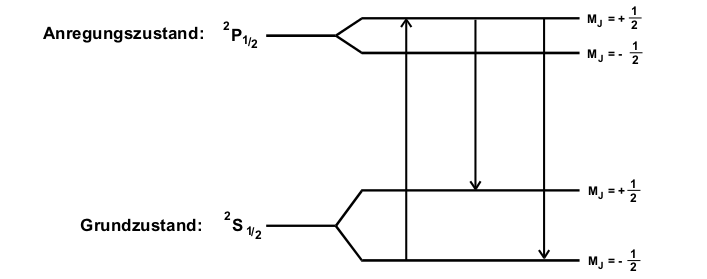
\includegraphics[width=12cm]{abb4.jpg}
	\caption{Übergänge unter Einfluss des rechtszikular-polarisierten Lichts \cite{V21}}
	\label{abb:abb4}
\end{figure}
Wird das ganze in einer Dampfzelle durchgeführt, kann die Intensität des durch die Dampfzelle hindurchtretenden Lichtes als Maß für die Besetzung des $^2S_\frac{1}{2}$, $M_\text{J}=-\frac{1}{2}$ Niveaus
benutzt werden. Die Tranzparenz nimmt während des Pumpvorgangs immer weiter zu, da die Wahrscheinlichkeit der Absorption des $D_1$-Lichtes immer mehr abnimmt. In Abbildung \ref{abb:abb5} ist dargestellt,
wie sich die Transparenz gegen die Zeit verändert.
\begin{figure}[H]
	\centering
	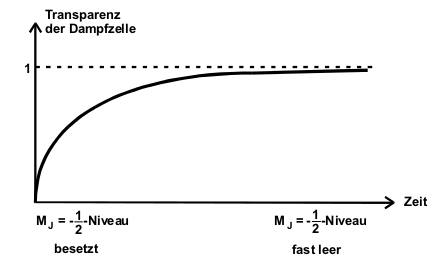
\includegraphics[width=10cm]{abb5.jpg}
	\caption{Tranzparenz in Abhängigkeit von der Zeit beim Einstrahlen von $D_1$-Licht \cite{V21}}
	\label{abb:abb5}
\end{figure}

\subsection{Präzissionsmessung der Zeeman-Aufspaltung}

Um die Aufspaltung des Zeeman-Effektes zu untersuchen, wird eine Methode der Hochfrequenzspektroskopie verwendet. Zuerst ist von relevanz, wie ein angeregtes Atom wieder in den Grundzustand übergeht. Dies
kann über zwei Prozesse geschehen, nämlich über die spontanen oder die induzierte Emission. Der Unterschied zwischen den beiden ist, dass bei der induzierten Emission ein Photon von außen
eingestrahlt werden muss, damit das Atom zurück in den Grundzustand fällt. Dabei muss die Energie des Photon genau dem Unterschied der beiden Niveaus entsprechen. Bei diesem Vorgang entstehen zwei Photonen,
deren Energie, Polarisation und Ausbreitungsrichtung gleich ist.
Welche der beiden Emissionen stattfindet hängt von der Energie der Photonen ab. Um die Übergänge ausmessen zu können muss überprüft werden, ob die spontane Emission die Messung beeinflusst.
Dazu wird die Anzahl der Atome $N_2$ im höheren Zusatand und die Anzahl der Atome $N_1$ im niedrigeren Zustand betrachtet.
Es ist zu beachten, dass die Zahl der pro Zeiteinheit übergehenden Atome proportional zur Dichte $u(v)$ der Quanten ist. Zusätzlich wird der Einstein-Koeffizient $B_{21}$ als Proportionalitätsfaktor benötigt.
Im thermischen Gleichgewicht gilt, dass genauso viele Photonen ausgesendet wie auch absorbiert werden. Somit kann die Gleichung
\begin{equation}
  N_2A_{21}+N_2B_{21}u(v)=N_1B_{12}u(v)
\end{equation}
aufgestellt werden. Dabei beschreibt der erste Summand die Anzahl der spontanen Emissionen, der zweite Teil die Anzahl der induzierten Emissionen und das Ergebnis die Anzahl aller Emissionen.
Weil die Emissionen durch Temperaturstrahlung induziert werden, kann mit Hilfe der Planckschen Formel eine Überganswahrscheinlichkeit vom Angeregten in den Grundzustand als
\begin{equation}
  A_{21}=\frac{8\pi h}{c^3}B_{12}\nu^3
\end{equation}
bestimmt werden. Der Einsteinkoeffizient ist in diesem Fall konstant. Nun ist eine $\nu^3$-Abhängigkeit der Frequenz zu erkennen. Da im Versuch die Frequenz der Zeeman-Übergänge im $1\,\text{MHz}$ Bereich,
die Frequenz der spontanen Übergänge jedoch im $380\,\text{THz}$ Bereich liegen, spielt die spontane Emission beim Ausmessen der Zeeman-Niveaus keine Rolle.

Zusätzlich kann mit der Apperatur des Magnetfeldd der Erde bestimmt werden. Dazu wird die Transparenz der Dampfzelle ohne äußeres Magnetfeld, also auch ohne Zeeman-Aufspaltung, gemessen.
Es ergibt sich der in Abbildung \ref{abb:abb6} dargestellte Verlauf der Kurve. Durch das Einstellen der Linien auf minimale Breite über die Spuelenströme, kann das Erdmagnetfeld in allen
Raumrichtungen abgelesen werden.

\begin{figure}[H]
	\centering
	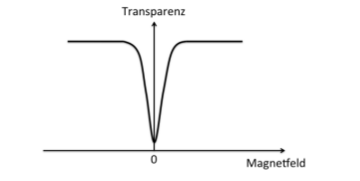
\includegraphics[width=8cm]{abb6.jpg}
	\caption{Tranzparenz der Dampfzelle ohne äußeres Magnetfeld \cite{V21}}
	\label{abb:abb6}
\end{figure}

Schließlich kann die für den Übergang zwischen den Zeeman-Niveaus benötigte Energie auch über die Tranzparenz der Dampfzelle bestimmt werden. Zuerst wird das untere Niveau komplett leer gepumpt und die Transparenz
erreicht ihr Maximum. Anschließend wird das $B$-Feld bis auf den Wert
\begin{equation}
  B_\text{m}=\frac{4\pi m_0}{e_0g_\text{J}}\nu
\end{equation}
erhöht, woddurch die induzierte Emission ausgelöst wird. Eingestrahltes $D_1$-Licht kann wieder absorbiert werden und somit nimmt die Transparenz im Resonanzfall wieder ab.
In Abbildung \ref{abb:abb7} ist der Verlauf der Messkurve dargestellt.

\begin{figure}[H]
	\centering
	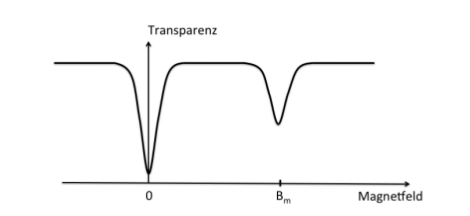
\includegraphics[width=8cm]{abb7.jpg}
	\caption{Tranzparenz der Dampfzelle im Resonanzfall \cite{V21}}
	\label{abb:abb7}
\end{figure}

Abschließend wird das Ganze für ein Atom mit Kernspin $I>0$ betrachtet. Hier tritt eine höhere Aufspaltung der Energieniveaus auf, das Prinzip zur Ausmessung dieser Niveaus bleibt dennoch das Gleiche.
Wieder müssen die Auswahlregeln beachtet werden. Aus diesem Grund kann auch in diesem Fall eine nicht-thermische Besetzung erzeugt werden, bei der die Dampfzelle transparent ist. Über den Resonanzfall kann
anschließend die Energie des Niveaus bestimmt werden. Dies erfolgt analog zu dem, wie es für den einfachen Fall erklärt worden ist.

\subsection{Quardratischer Zeemann-Effekt}
Wenn die Feldstärke $\vec B$ des Magnetfeldes groß wird, müssen bei der Berechnung der Übergangsenergie $U_\text{HF}$ zwischen zwei Energieniveaus quadratische Terme berücksichtigt werden. Mit der Hyperfeinstrukturkaufspaltung $\Delta E_\text{Hy}$  zwischen den Energieniveaus F und F+1 berechtet sich die Übergangsenergie durch
\begin{equation}
  U_\text{HF}=g_\text{F}\mu_\text{B}B+g_\text{F}^2\mu^2_\text{B}B^2\frac{1-2M_\text{F}}{\Delta E_\text{Hy}}.
\end{equation}

\subsection{Transistente Effekte}
Wenn nun das Hochfrequenzfeld nicht mehr dauerhaft eingestellt ist, sondern schnell an- und ausgeschaltet wird, verändert sich das Verhalten des Pumpsystems. Das Magnetfeld und das Hochfrequenzfeld werden beide auf die Lamorfrequenz
\begin{equation}
  \omega_0=2\pi\nu_0=\underbrace{g_\text{f}\frac{\mu_0}{h}}_{:=\gamma}B_0
\end{equation}
eingestellt, $\gamma$ heißt gyromagnetisches Verhältnis.

Wenn die Amplitude des Hochfrequenzfeldes wesentlich kleiner ist, als die des statischen Feldes, präzediert der Vektor $\vec F$ wie in Abbildung \ref{abb:8} um die Feldrichtung $\vec{B}$ des statischen Feldes.
Im Koordinatesystem des sich drehenden $\vec{F}$-Vektors setzt sich das effektive Magnetfeld $\vec{B}_\text{eff}$ aus dem statischen Magnetfeld und dem Hochfrequenzfeld zusammen:
\begin{equation}
  \vec{B}_\text{eff}=\vec{B}+\frac{\omega}{\gamma}.
\end{equation}
In diesem Koordinatensystem präzediert $\vec{F}$ mit der Lamor-Frequenz $\nu=\gamma \vec{B}_\text{RF}$, also mit einer Periode von $T=\frac{1}{\gamma B_\text{RF} }$. Daher gilt bei resonantem Hochfrequenzfeld die Relation
\begin{equation}
  \frac{T_\text{87}}{T_\text{85}}=\frac{\gamma_\text{85}}{\gamma_\text{87}}
\end{equation}
zwischen den Perioden der Isotope. (ich habe keine ahnung, warum das daraus folgt. im skript sind noch komische rechenschritte, aber ich denke nicht, dass die ins protokoll gehören........................................)
\begin{figure}[H]
	\centering
	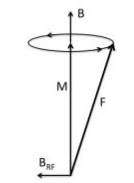
\includegraphics[width=3.5cm]{abb8.jpg}
	\caption{Vektor $\vec F$ präzediert um die Feldrichtung $\vec{B}$ \cite{V21}}
	\label{abb:8}
\end{figure}
